% =====================================================================
% Snippet: summary-bar.tex
% =====================================================================
% USAGE: Bottom pipeline summary bar — N labels separated by arrows.
% This is what test-gat figure has at the bottom:
%   Molecule -[GAT]-> (A, X) -[GAT]-> α_ij Weighted -[Multi-head]-> ...
%
% Copy %% COPY-START / END, replace:
%   - stages: \def\sumdata{label/edge, label/edge, ...}
%     - label: stage name
%     - edge: arrow label text (empty = no label)
%   - origin_x, origin_y
%   - item_gap: spacing between stage centers (default 2.5)
% =====================================================================

\documentclass[tikz,border=10pt]{standalone}
\usepackage{xcolor,tikz}
\usetikzlibrary{positioning,calc,arrows.meta,bending}

\definecolor{acaGreyLine}{HTML}{606060}
\definecolor{acaGreyFill}{HTML}{F0F0F0}
\definecolor{acaPurpleLine}{HTML}{6E3FA0}

\tikzset{
  sum stage/.style={
    rectangle, rounded corners=3pt,
    fill=acaGreyFill, draw=acaGreyLine, line width=0.5pt,
    font=\scriptsize, text=acaGreyLine,
    inner sep=4pt, minimum height=0.5cm,
  },
  sum arrow/.style={
    -{Stealth[length=4pt 1.0, width'=0pt 0.5]},
    line width=0.6pt, color=acaPurpleLine,
    shorten >=1pt, shorten <=1pt,
  },
}

\begin{document}
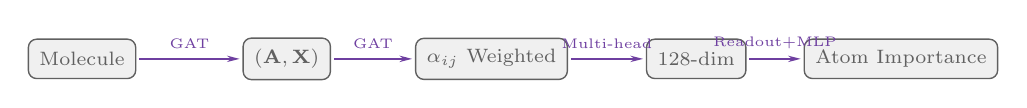
\begin{tikzpicture}

%% COPY-START =========================================================
% Note: \foreach can't handle entries with `,` inside math, so we
% hard-code 5 entries. For your figure, edit labels + edge texts below.

\def\xO{0}
\def\yO{0}
\def\itemGap{2.6}

% --- STAGES ---
\node[sum stage] (sb1) at (\xO + 0*\itemGap, \yO) {Molecule};
\node[sum stage] (sb2) at (\xO + 1*\itemGap, \yO) {$(\mathbf{A}, \mathbf{X})$};
\node[sum stage] (sb3) at (\xO + 2*\itemGap, \yO) {$\alpha_{ij}$ Weighted};
\node[sum stage] (sb4) at (\xO + 3*\itemGap, \yO) {128-dim};
\node[sum stage] (sb5) at (\xO + 4*\itemGap, \yO) {Atom Importance};

% --- ARROWS WITH EDGE LABELS ---
\draw[sum arrow] (sb1.east) -- (sb2.west)
  node[midway, above, font=\tiny, color=acaPurpleLine] {GAT};
\draw[sum arrow] (sb2.east) -- (sb3.west)
  node[midway, above, font=\tiny, color=acaPurpleLine] {GAT};
\draw[sum arrow] (sb3.east) -- (sb4.west)
  node[midway, above, font=\tiny, color=acaPurpleLine] {Multi-head};
\draw[sum arrow] (sb4.east) -- (sb5.west)
  node[midway, above, font=\tiny, color=acaPurpleLine] {Readout+MLP};

%% COPY-END ===========================================================

\end{tikzpicture}
\end{document}
